\documentclass[12pt]{article}
 
\usepackage[margin=1in]{geometry} 
\usepackage{amsmath,amsthm,amssymb,outlines}
\usepackage{graphicx}
\usepackage{tikzsymbols}
\newtheorem{definition}{Definition}
\newtheorem{question}{Question}
\newtheorem{answer}{Answer}
\newtheorem{example}{Example}
\newtheorem{theorem}{Theorem}
\newenvironment{statement}[2][Statement]{\begin{trivlist}
\item[\hskip \labelsep {\bfseries #1}\hskip \labelsep {\bfseries #2.}]}{\end{trivlist}}

\begin{document}
 
\title{Complex Analysis Notes} 
\author{Dahlen Elstran} 
\maketitle

\section*{Chapter 1: Preliminaries to Complex Analysis}

\subsection*{1.3: Integration Along Curves}

\begin{definition}
  A \textbf{parametrized curve} is a function $\gamma(t)$ which maps a closed interval $[a,b] \subset \mathbb{R}$ 
  to the complex plane.
\end{definition}

I like to think about parametrized curves as just a dictionary taking a real number and outputting a complez number. 
The following is an example of a parametrized cuve $\gamma(t)$ that goes from $[0,1]$, where every $z_i$ is another output of a $t$. 
\begin{center} 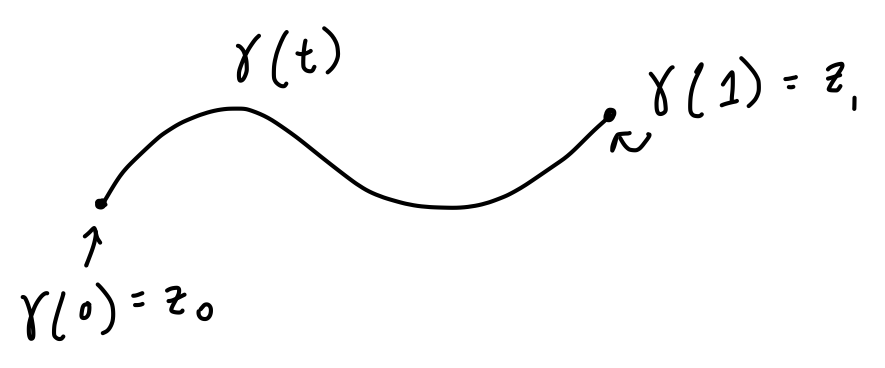
\includegraphics[scale=.3]{8150.1.png} \end{center}

\begin{definition}
  A parametrized curve $\gamma(t)$ is \textbf{smooth} if $\gamma'(t)$ exists, is continuous on $[a,b]$, and is nonzero for $[a,b]$.
\end{definition}

So a curve that has no "sharp points" or min/max's for all of $[a,b]$ is smooth on $[a,b]$.

Note that also in this definition of smooth, we define $\gamma'(a)$ as the one-sided linit from the right, and vice versa for $\gamma'(b)$. 

\begin{definition}
  A parametrized curve $\gamma(t)$ is \textbf{piecewise-smooth} if $\gamma$ is continuous on $[a,b]$ and if it is smooth in intervals $[a, a_1], \dots [a_{n-1},a_n = b]$.
\end{definition}

So if a curve has a continuous derivative but has max's and min's, it is piecewise-smooth. 

\begin{question}
  If a smooth surve has a nonzero derivative for all $[a,b]$, wouldn't maxes and mins make it impossible to find an interval $[a_i,a_{i+1}]$ such that
  there is no zero at all?
\end{question}

\begin{answer}
  That's where the one-sided limits come in, because the derivative is only zero at the exact point. When you break the intervals up at all the maxes and mins, 
  that exact point is not evaluated, just the (nonzero) one sided limits of them.
\end{answer}

\begin{definition}
  Two parametrizations $z: [a,b] \to \mathbb{C}$ and $\bar{z}: [c,d] \to \mathbb{C}$ are \textbf{equivalent} if there exists a continuously differentiable bijection
  from $[c,d]$ to $[a,b]$ so that $t'(s) > 0$ and $\bar{z}(s)=z(t(s))$.
\end{definition}

So two parametrizations are equivalent if they describe the same curve (and therefore same set of points), but parametrize them differently, but with the same orientation. 
Essentially, the two parametrizations just go at different "speeds" along the curve in the same direction. Note that if you're looking at a curve $\gamma$, $\gamma^-$ 
represents the same curve, going the opposite direction. 

\begin{definition}
  The familt of all parametrizations that are equivalent to $z(t)$ determines a \textbf{smooth curve} $\gamma \subset \mathbb{C}$
\end{definition}

This is just saying all these parametrizations are equivalent along thier curve with orientation, so a smooth curve is just a curve with orientation and parametrization. 

\begin{definition}
  A (piecewise) smooth curve is called \textbf{closed} if $z(a)=z(b)$
\end{definition}

Basically, the curve is any loop. 

\begin{example}
  The following is a closed curve, namely a circle, centered at $z_0$ with radius $r$:
  \begin{align*}
    C_r(z_0) = \{ z \in \mathbb{C} : |z-z_0| = r\}
  \end{align*}
  The positive orientation (counterclockwise) is the parametrization $z(t) = z_0 + re^{it}$, where $t \in [0,2\pi]$. 
\end{example}

This parametrization moves around the circle (because $e^{it} = \cos(t) + i \sin(t)$) with radius $r$. 
Clearly, $t \in \mathbb{R}$ and maps to a complex number. 

\begin{definition}
  We define the integral of a continuous function $f$ along a smooth curve $\gamma$ by 
  \begin{align*}
    \int_{\gamma}f(z)dz = \int^b_a f(z(t))z'(t).
  \end{align*}
\end{definition}

First note that in $\mathbb{R}$, we think of integration as the area under a curve, but this can be more generally seen as adding up 
all the $f(x)$ values at each $x$. With this lens, we can think of complex integration the same way: we want to add up all the $f(z)$ for an 
infinite number of $z$. We can integrate along a curve (with parametrization) so that we can put $z$ in terms of $t$ instead, so that we are integrating 
real numbers instead of complex ones. 

\par The textbook shows that this is independent of the parametrization defined on the curve, but conceptually, it shouldn't matter how "fast" you 
move down a curvwe, you are still adding up the same values. 

\par If the curve is piecewise-smooth and not smooth, the integral is simply broken up into the integrals of each smooth interval. 

\begin{definition}
  The \textbf{length} of the smooth curve $\gamma$ is 
  \begin{align*}
    \text{length}(\gamma)=\int^a_b |z'(t)|dt.
  \end{align*}
\end{definition}

\begin{question}
  What does this mean? What is $z'(t)$? Why does this work?
\end{question}

You can pull complex scalars out of the integral, as well as adding and subtracting in the integral like you can in the real plane. 
The negative integral is just going over the curve in the reverse direction. 

\begin{theorem}
  \begin{align*}
    |\int_{\gamma} f(z) dz | \leq \sup_{z \in \gamma}
  \end{align*}
\end{theorem}

FINISH THIS

\section*{Chapter 2: Cauchy's Theoem and It's Applications}



\end{document}
